%
% ==--------------------------------------------------------------------------==
% 
% Build for XeLaTeX !
% 
% В папку tex-source необходимо поместить файл sign.png (800x800) с подписью.
% 
% ==--------------------------------------------------------------------------==

\documentclass[12pt, a4paper]{report}
\usepackage[utf8x]{inputenc}
\usepackage[english,russian]{babel} 
\usepackage{graphicx} % Для вставки рисунков
\usepackage{indentfirst}
% \usepackage{hyperref}
\usepackage{setspace} 
% \usepackage{tikz}
\usepackage{fontspec} % Изменение шрифтов
\usepackage{makecell} % Переносы в таблицах
\usepackage{etoolbox} % Макет оглавнения http://ctan.org/pkg/etoolbox
\usepackage{ragged2e} % Для выравнивания по ширине
\usepackage{listings} % Для листингов кода
\usepackage{xcolor} % Для цвета в листингах

\usepackage{tex-system} 

% ==--------------------------------------------------------------------------==
%                                                                
% Переменные
% 
\def\workName{Лабораторная работа № }
\def\workSubname{subnamePlaceholder}
\def\myName{Коренев Д.Н.}
\def\myGroup{КБ-211}
\def\myTeacher{namePlaceholder}
\def\myCity{Белгород}
\def\year{2023}
% 
% 
% \Переменные
% 
% ==--------------------------------------------------------------------------==

% ==--------------------------------------------------------------------------==
% 
% Макросы
% 
% Секция без номера, в центре, в оглавлении
\newcommand{\middleSection}[1]{
    \addcontentsline{toc}{section}{#1}
    \section*{\hfil#1\hfil}
}
% \Макросы
% 
% ==--------------------------------------------------------------------------==

\begin{document}
% ==--------------------------------------------------------------------------==
% 
% Титульный лист
% 
% 
% top of the page
\begin{center}
    \textbf{Федеральное государственное бюджетное образовательное учреждение
    высшего образования ''Белгородский государственный технологический
    университет им. В.Г. Шухова''}
\end{center}
% 
\vspace{0.1cm}
% 
\begin{center}
    Кафедра программного обеспечения вычислительной техники и
    автоматизированных систем
\end{center}
% 
\vspace{3cm}
% 
\begin{center}
    \textbf{\workName{}} \\
    \workSubname{}
\end{center}
% 
% align right
\vspace{4cm}
\begin{flushright}
    \begin{minipage}{0.5\textwidth}
        \begin{flushleft}
            Выполнил: \\
            Студент группы \myGroup{} \\
            % use this vspace or signature
            % \vspace{3.6cm}
            \includegraphics[scale=0.35]{sign}\\
            \vspace*{-1.25cm}\underline{\hspace{3cm}} \myName{}\\
            \vspace{0.1cm}
            Принял: \\
            \vspace{1cm}
            \underline{\hspace{3cm}} \myTeacher{}
            
        \end{flushleft}
    \end{minipage}
\end{flushright}

\thispagestyle{empty} % disable page numbering on first page
\begin{center}
    \vfill \myCity{} \year{} % text at the bottom of the page
\end{center}

\newpage
% 
% \Титульный лист
% 
% ==--------------------------------------------------------------------------==

% ==--------------------------------------------------------------------------==
% 
% Основная часть
% 
\tableofcontents
\newpage

\sloppy

\middleSection{Пример абзаца}

Lorem ipsum dolor sit amet, consectetur adipiscing elit. Proin porttitor dictum 
dui, eu aliquet sem laoreet id. Curabitur non nulla mauris. In hac habitasse 
platea dictumst. Maecenas ligula diam, porta rhoncus libero in, commodo 
venenatis turpis.

\textbf{Lorem ipsum dolor sit amet, consectetur adipiscing elit. 
Proin porttitor dictum 
dui, eu aliquet sem laoreet id. Curabitur non nulla mauris. In hac habitasse 
platea dictumst. Maecenas ligula diam, porta rhoncus libero in, commodo 
venenatis turpis.}

\textit{Lorem ipsum dolor sit amet, consectetur adipiscing elit. 
Proin porttitor dictum 
dui, eu aliquet sem laoreet id. Curabitur non nulla mauris. In hac habitasse 
platea dictumst. Maecenas ligula diam, porta rhoncus libero in, commodo 
venenatis turpis.}

\texttt{Lorem ipsum dolor sit amet, consectetur adipiscing elit. 
Proin porttitor dictum 
dui, eu aliquet sem laoreet id. Curabitur non nulla mauris. In hac habitasse 
platea dictumst. Maecenas ligula diam, porta rhoncus libero in, commodo 
venenatis turpis.}



\middleSection{Пример списка}
\begin{itemize}
    \item Первый
    \item Второй
    \item Третий
\end{itemize}

\middleSection{Пример нумерованного списка}
\begin{enumerate}
    \item Первый
    \item Второй
    \item Третий
\end{enumerate}

\middleSection{Пример кода}
\begin{lstlisting}[language=Python]
    import numpy as np
    
    def incmatrix(genl1,genl2):
        m = len(genl1)
        n = len(genl2)
        M = None # to become the incidence matrix
        VT = np.zeros((n*m,1), int) # dummy variable
        
        # compute the bitwise xor matrix
        M1 = bitxormatrix(genl1)
        M2 = np.triu(bitxormatrix(genl2),1) 

        for i in range(m-1):
            for j in range(i+1, m):
                [r,c] = np.where(M2 == M1[i,j])
                for k in range(len(r)):
                    VT[(i)*n + r[k]] = 1;
                    VT[(i)*n + c[k]] = 1;
                    VT[(j)*n + r[k]] = 1;
                    VT[(j)*n + c[k]] = 1;
                    
                    if M is None:
                        M = np.copy(VT)
                    else:
                        M = np.concatenate((M, VT), 1)
                    
                    VT = np.zeros((n*m,1), int)

                    print('Some string for example')
        return M
\end{lstlisting}

\begin{lstlisting}[language=CSharp]     
    class Program
    {
        static void Main(string[] args)
        {
            int num1, num2, sum;
            Console.WriteLine("Calculate the sum of two numbers:");
            Console.Write("Input number1:");
            num1 = Convert.ToInt32(Console.ReadLine());
            Console.Write("Input number2:");
            num2 = Convert.ToInt32(Console.ReadLine());
            sum = num1 + num2;
            Console.Write("Result:"+sum);

            Console.ReadKey();
        }
    }
\end{lstlisting}

\begin{lstlisting}[language=Rust]
    // Unlike C/C++, there's no restriction on the order of function definitions
    fn main() {
        // We can use this function here, and define it somewhere later
        fizzbuzz_to(100);
    }

    // Function that returns a boolean value
    fn is_divisible_by(lhs: u32, rhs: u32) -> bool {
        // Corner case, early return
        if rhs == 0 {
            return false;
        }

        // This is an expression, the `return` keyword is not necessary here
        lhs % rhs == 0
    }

    // Functions that "don't" return a value, actually return the unit type `()`
    fn fizzbuzz(n: u32) -> () {
        if is_divisible_by(n, 15) {
            println!("fizzbuzz");
        } else if is_divisible_by(n, 3) {
            println!("fizz");
        } else if is_divisible_by(n, 5) {
            println!("buzz");
        } else {
            println!("{}", n);
        }
    }

    // When a function returns `()`, the return type can be omitted from the
    // signature
    fn fizzbuzz_to(n: u32) {
        for n in 1..=n {
            fizzbuzz(n);
        }
    }
\end{lstlisting}

\middleSection{Пример цитаты}
Далее приведена цитата из Lorem ipsum.
\begin{quotation}
    Lorem ipsum dolor sit amet, consectetur adipiscing elit. Proin porttitor 
    dictum 
    dui, eu aliquet sem laoreet id. Curabitur non nulla mauris. In hac habitasse 
    platea dictumst. Maecenas ligula diam, porta rhoncus libero in, commodo 
    venenatis turpis.
\end{quotation}
Текст сразу после цитаты.

Следующий абзац.

\middleSection{Пример рисунка}
\begin{figure}[ht]
    \centering
    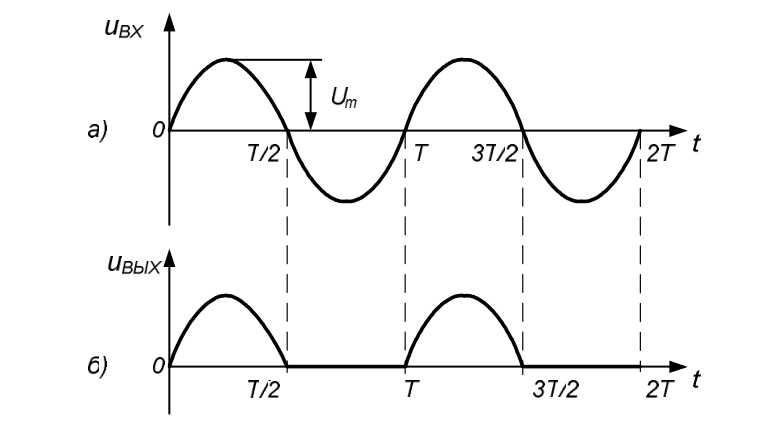
\includegraphics[width=\textwidth]{pictureExample}
    \caption{Пример текста под рисунком}
    \label{fig:pictureExample}
\end{figure}

На странице \pageref{fig:pictureExample} на рисунке \ref{fig:pictureExample} показан пример рисунка. Он самостоятельно
встраивается в текст между абзацами.


\middleSection{Пример таблицы}
\begin{table}[h]
    \centering
    \begin{tabular}{|l|c|r|}
        \hline
        \textbf{Заголовок 1} & \textbf{Заголовок 2} & \textbf{Заголовок 3} \\ \hline
        1                    & 2                    & 3                    \\ \hline
        4                    & 5                    & 6                    \\ \hline
        7                    & 8                    & 9                    \\ \hline
        7                    & 8                    & 9                    \\ \hline
        7                    & 8                    & 9                    \\ \hline
        7                    & 8                    & 9                    \\ \hline
        7                    & 8                    & 9                    \\ \hline
        7                    & 8                    & 9                    \\ \hline
        7                    & 8                    & 9                    \\ \hline
        7                    & 8                    & 9                    \\ \hline
        7                    & 8                    & 9                    \\ \hline
        7                    & 8                    & 9                    \\ \hline
    \end{tabular}
    \caption{Пример таблицы}
    \label{tab:tableExample}
\end{table}
\clearpage

\middleSection{Пример формул}
\begin{equation}
    \label{eq:1}
    f(x) = \alpha_1 z_1+\alpha_2 z_2+\ldots+\alpha_n z_n
\end{equation}
\begin{equation}
    \label{eq:2}
    \beta_1 z_1+\beta_2 z_2 \geq 0
\end{equation}
\begin{equation}
    \label{eq:3}
    \vec{x} = \{x_1, x_2, \ldots, x_n\}
\end{equation}
\begin{equation}
    \label{eq:4}
    \left\{
    \begin{array}{c}
        a_{11} x_1 + a_{12} x_2 \leq b_1 \\
        a_{21} x_1 + a_{22} x_2 \leq b_2 \\
        \ldots \\
        a_{m1} x_1 + a_{m2} x_2 \leq b_m \\
    \end{array}
    \right.
\end{equation}

Выражения \ref{eq:1}, \ref{eq:2}, \ref{eq:3}, \ref{eq:4} показывают примеры 
формул.
% 
% \Основная часть
% 
% ==--------------------------------------------------------------------------==

% ==--------------------------------------------------------------------------==
% 
% Приложения
% 
\clearpage
\middleSection{Приложения}
\subsection*{Приложение 1. Пример приложения.}

На линейной диаграмме RGB показано точное от 0 до 255 и процентное от 0 до 
100\% содержание цветов (красного, зелёного и синего) в 98AB16. На круговой 
диаграмме RGB показано относительное содержание цветов в 98AB16.

\subsection*{Приложение 2. Пример приложения.}

На линейной диаграмме CMYK показано только процентное от 0 до 100\% 
содержание цветов (голубого, пурпурного, жёлтого и чёрного) в 98AB16. 
На круговой диаграмме CMYK показано относительное содержание цветов в 98AB16.

\subsection*{Приложение 3. Пример листинга.}
\lstinputlisting[language=Python]{./tex-source/codeExample.py}
% 
% \Приложения
% 
% ==--------------------------------------------------------------------------==

\end{document}
